\graphicspath{{chapters/contents/sessio_03/images/}}
\section{La cola que uneix la física clàssica}

Recordes quan fullejàvem el llibre de Física i ens preguntàvem per què estudiem juntes coses que, d'entrada, no semblen tenir gaire a veure?

Electricitat, calor, moviment, so, llum...

Quina relació hi pot haver entre un glaçó que es desfà, un endoll o el soroll d'una moto que passa pel carrer espantant tots els gossos del barri?

Doncs sí que n'hi ha una. I va costar bastant adonar-se'n.

\subsection{Cadascú fent la seva física}

El 1687, Newton va publicar els \textit{Principia} i va establir les bases de la mecànica clàssica. La cosa tenia mèrit: amb unes mateixes lleis podies descriure tant el moviment d'un objecte que cau com el dels planetes.

De sobte, una part enorme del món físic començava a tenir una estructura comuna.

Mentrestant, però, altres científics continuaven treballant pel seu compte amb la calor, l'electricitat, els fluids, la llum...

Tothom anava fent.

Faltava trobar alguna cosa que connectés totes aquelles peces.

\subsection{Joule i una cerveseria sorprenentment útil}

James Prescott Joule va néixer el 1818 en una família que tenia una pròspera fàbrica de cervesa a prop de Manchester.

De jove va tenir com a professor particular John Dalton. Sí, \textit{el Dalton dels àtoms}. Ja parlarem del senyor Dalton, que també dona bastant tema de conversa.

Però Joule també havia de treballar al negoci familiar. El seu pare, Benjamin Joule, tenia una empresa que funcionava prou bé i semblava bastant raonable que el fill hi dediqués part del temps.

Això podia haver estat una molèstia.

Però resulta que una fàbrica de cervesa té termòmetres, dipòsits, aigua, motors, mecanismes, tubs i tota mena de coses que, si tens una certa tendència a fer experiments, s'assemblen sospitosament a un laboratori.

Joule va començar a estudiar la relació entre moviment, electricitat i calor. Va fer passar corrent per fils submergits en aigua i va mesurar com augmentava la temperatura. També va fer experiments en què unes masses que queien feien girar unes pales dins d'un recipient amb aigua.

\begin{figure}[H]
    \centering
    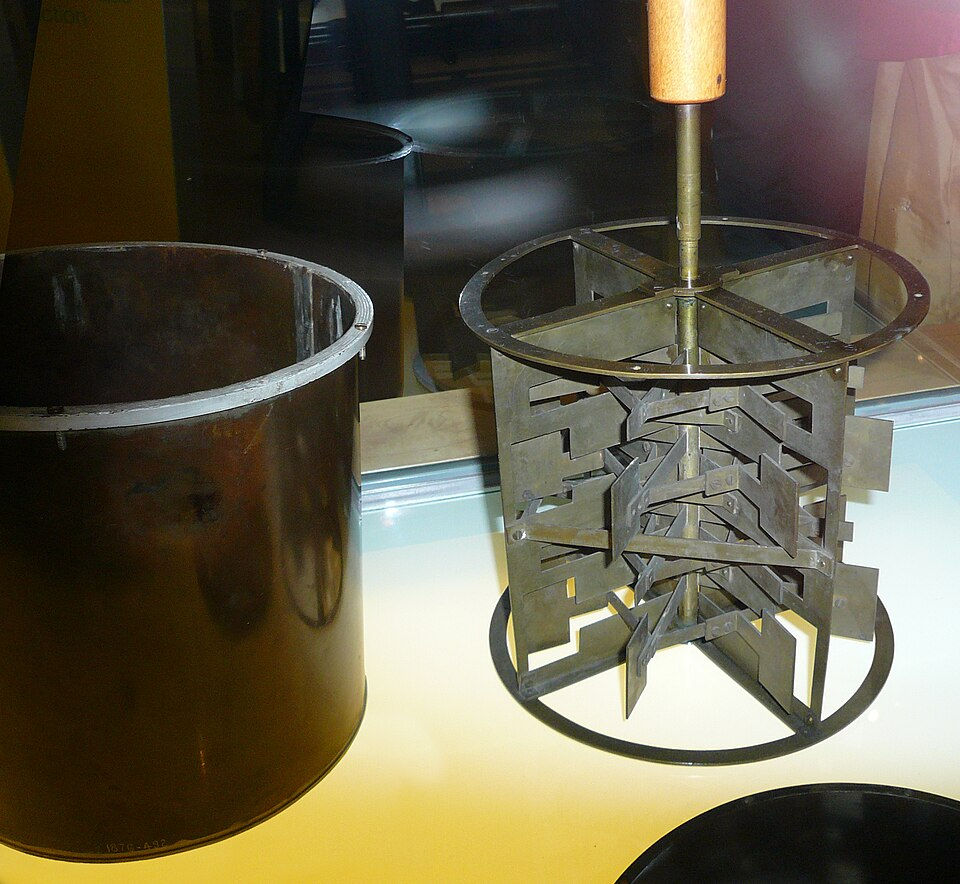
\includegraphics[width=0.75\linewidth]{joule.jpg}
    \caption{Aquestes són les pales amb què s’entretenia a les tardes "el tete" Joule. I, mentrestant, estava descobrint una cosa bastant important. Foto: Dr. Mirko Junge - Wikimedia Commons, CC BY 3.0.}
\end{figure}

Les pales agitaven l'aigua i l'aigua s'escalfava.

Si augmentava el treball mecànic realitzat, augmentava també l'escalfament.

\textit{Anomenem treball mecànic a l'energia que transferim quan una força provoca un desplaçament. Dit més planerament: si fas força sobre alguna cosa i aconsegueixes moure-la, estàs fent treball mecànic.}

I si aïllava bé el recipient, era cada vegada més difícil explicar aquell augment de temperatura dient simplement que la calor havia entrat de fora.

Joule estava trobant una equivalència entre coses que fins aleshores s'havien estudiat gairebé per separat: el treball mecànic podia convertir-se en calor, i aquesta conversió es podia mesurar.

Alguna cosa semblava estar passant d'una forma a una altra.

A aquella cosa acabarem anomenant-la \textbf{energia}.

\subsection{Una cosa que apareix a tot arreu}

Encara no hem definit del tot què és l'energia. De moment, però, ja podem veure una cosa important: apareix per tot arreu.

Podem transformar:
\[
\text{moviment}
\longrightarrow
\text{electricitat}
\]
\[
\text{electricitat}
\longrightarrow
\text{calor}
\]
\[
\text{energia química}
\longrightarrow
\text{moviment}
\]
\[
\text{moviment}
\longrightarrow
\text{so}
\]
\[
\text{llum}
\longrightarrow
\text{calor}
\]
I podem continuar una bona estona.

L'energia és, en certa manera, la cola que permet entendre per què branques de la física que semblaven independents formen part del mateix edifici.

Però això obre immediatament una pregunta bastant grossa:
\begin{quote}
D'on surt aquesta energia? Podem crear-ne? Pot simplement desaparèixer?
\end{quote}
El llenguatge quotidià aquí ajuda poc.

Quan diem que alguna cosa ``ens ha consumit tota l'energia'', no vol dir que l'energia hagi desaparegut de l'univers. Normalment vol dir que l'hem gastada fent alguna cosa, útil o absurda, i ara preferiríem estar estirats al sofà.

\subsection{Entra Helmholtz}

A mitjan segle XIX encara era habitual trobar explicacions segons les quals els éssers vius disposaven d'alguna mena de ``força vital'' especial, diferent de les forces que actuaven sobre la matèria normal.

Una pedra era física. Un cangur (per buscar un exemple d’alguna cosa viva), aparentment, necessitava alguna cosa més. Hermann von Helmholtz, que era metge i fisiòleg a més de físic, no ho veia gaire clar.

Estudiant el funcionament dels músculs i el metabolisme va arribar a una idea molt més simple: els organismes també transformaven energia. L'energia química dels aliments podia acabar convertida en moviment, calor i altres formes d'energia.

El 1847 va publicar \textit{Über die Erhaltung der Kraft}, un treball fonamental en la formulació general del principi de conservació de l'energia.

La idea essencial era aquesta:
\[
\boxed{
\text{En un sistema aïllat, l'energia total es conserva.}
}
\]

Pot canviar de forma.

Pot passar d'un objecte a un altre.

Pot acabar repartida de manera tan poc útil que recuperar-la sigui pràcticament impossible.

Però no apareix del no-res ni simplement desapareix.

\subsection{El negoci perfecte que mai no va funcionar}

POV: inventes una màquina que consumeix una unitat d’energia i en produeix deu.

Fantàstic.

Connecto la sortida a deu màquines iguals, i ja estic traient $100$ unitats d'energia.:
\[
1 \longrightarrow 10 \longrightarrow 100
\]
Ara connecto deu màquines més a cadascuna:
\[
1 \longrightarrow 10 \longrightarrow 100 \longrightarrow 1000
\]

Amb unes quantes rondes ja no necessito ni acabar aquesta classe. Negoci rodó.

Malauradament, la física té la desagradable mania de revisar els comptes.

Una màquina capaç de produir contínuament més energia de la que rep seria una forma de \textbf{mòbil perpetu}. I violaria el principi de conservació de l'energia, del qual ja hem parlat a l'apartat anterior.

Fins ara ningú no ha pogut demostrar que una d’aquestes màquines funcioni de veritat. I si algú n’ha construït una, de moment ho està portant amb una discreció admirable.
\vfill
\newpage

\begin{figure}[H]
    \centering
    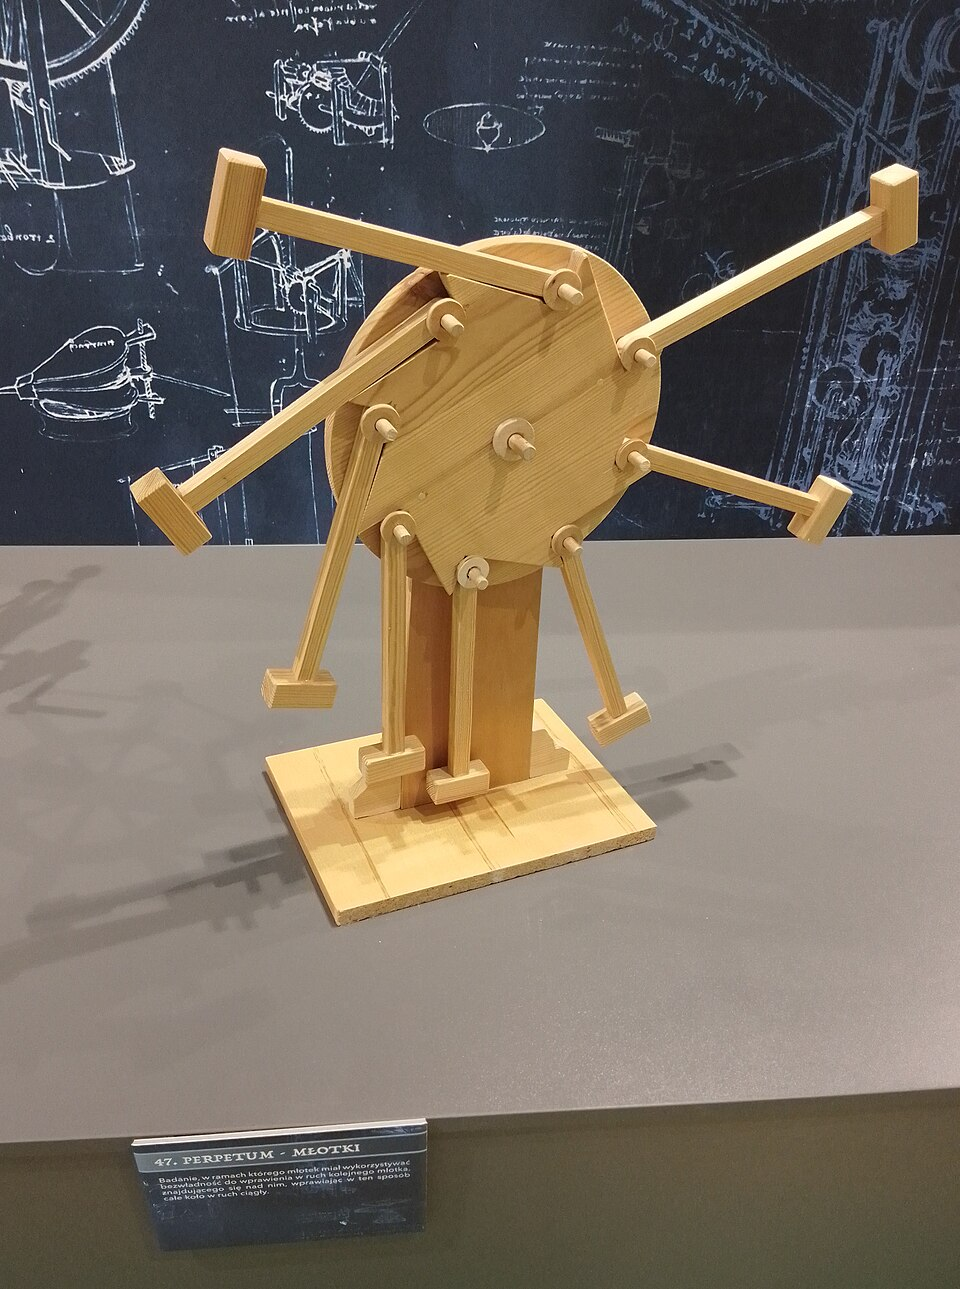
\includegraphics[width=0.75\linewidth]{perpetuum_mobile.jpg}
    \caption{Reproducció d’un mòbil perpetu atribuït a Leonardo da Vinci. Foto: Brandmeister (Togrul Safarov) -Wikimedia Commons, Creative Commons Zero, Public Domain Dedication.}
\end{figure}

Així que, si algú us presenta una màquina que genera energia gratis per sempre, hi ha dues possibilitats.

O acaba de trencar una de les lleis més ben comprovades de la física...

o convé mirar una mica millor on està connectat el cable.

\subsection{El petit desastre de les unitats}

Hi havia, a més, un problema pràctic.

La mecànica, la calor, l'electricitat i la química s'havien desenvolupat durant molt de temps de manera força independent. Cadascuna havia creat les seves pròpies maneres de mesurar les coses.

Quan finalment vam entendre que moltes d'aquelles quantitats representaven formes de la mateixa magnitud, ja teníem un bon assortiment d'unitats.

Una situació semblant a descobrir que tothom mesura longituds, però uns ho fan en metres, uns altres en polzades i algú ha decidit que la longitud de tres cavalls posats en fila també era una opció acceptable.

Per posar una mica d’ordre entre totes aquestes unitats, es va establir un sistema comú de mesures que avui coneixem com a \textbf{Sistema Internacional d’Unitats}. En aquest sistema, la unitat estàndard d’energia és el \textbf{joule} o \textbf{julio}, amb símbol:
\[
\mathrm{J}
\]

Endevina a qui volien homenatjar amb el nom.

Algunes unitats d'energia que encara podem trobar són:


\begin{center}
\scriptsize
\renewcommand{\arraystretch}{1.35}
\setlength{\tabcolsep}{3pt}
\begin{tabularx}{\linewidth}{
|>{\centering\arraybackslash}p{0.9cm}
|>{\raggedright\arraybackslash}p{1.45cm}
|>{\raggedright\arraybackslash}X
|>{\centering\arraybackslash}p{1.65cm}|}
\hline
\textbf{Unitat} &
\textbf{Nom} &
\textbf{Ús habitual} &
\textbf{Equivalència} \\
\hline

$\mathrm{cal}$ &
caloria &
Termodinàmica i química &
$4{,}184\ \mathrm{J}$ \\
\hline

$\mathrm{kcal}$ &
quilocaloria &
Termodinàmica i alimentació &
$4184\ \mathrm{J}$ \\
\hline

$\mathrm{kWh}$ &
quilowatt hora &
Electricitat i enginyeria &
$3{,}6\times10^{6}\ \mathrm{J}$ \\
\hline

$\mathrm{erg}$ &
erg &
Sistema CGS; física clàssica i astrofísica &
$10^{-7}\ \mathrm{J}$ \\
\hline

$\mathrm{eV}$ &
electró-volt &
Física atòmica, nuclear i de partícules &
$1{,}60\times10^{-19}\ \mathrm{J}$ \\
\hline

\end{tabularx}
\end{center}

Aquesta confusió ha sobreviscut perfectament fins als nostres dies. No semblava disposada a perdre's la festa.

\subsection{D'on surt un joule?}

La longitud, el temps i la massa són exemples de \textbf{magnituds fonamentals}.

Les anomenem així perquè no les definim com una combinació d'altres magnituds més bàsiques.

En canvi, altres magnituds sí que es poden construir a partir d'aquestes. Per exemple:

\[
\text{velocitat}=\frac{\text{distància}}{\text{temps}}
\]
o
\[
\text{volum}=\text{alt × ample × llarg} = \text{longitud}^{3} 
\]

L'energia és una \textbf{magnitud derivada}. De fet, quan escrivim les seves unitats, hi apareix una combinació de les tres magnituds fonamentals que ja coneixem: \textbf{massa, longitud i temps}.

En unitats fonamentals del Sistema Internacional:

\[
1\ \mathrm{J}
=
1\ \mathrm{kg}
\frac{\mathrm{m}^{2}}{\mathrm{s}^{2}}.
\]

Per fer-nos una idea, una poma d'uns $100\ \mathrm{g}$ que cau des d'aproximadament un metre arriba al terra amb prop d'un joule d'energia.

No cal complicar-ho gaire més, de moment. La poma cau, arriba amb aquella energia i, quan toca a terra, aquesta es reparteix entre el cop, el so, una mica de calor, petites deformacions...

L'energia continua allà. La poma, segons com hagi caigut, potser ja no tant.

L'energia continua existint.

La poma potser ja no està tan contenta.

I no, amb un joule no carregarem un mòbil un $1\,\%$. Ni de lluny. Un telèfon necessita desenes de milers de joules per carregar completament la bateria.

\subsection{I com sabem que una cosa és energia?}

Arribats aquí ja tenim una pista bastant bona.

Si una quantitat es pot transformar de manera mesurable en calor, moviment, llum, so o electricitat, i podem seguir els comptes sense que aparegui ni desaparegui res pel camí, estem parlant d'energia.

No n'hi ha prou, per tant, amb dir que alguna cosa ``té energia''. Aquesta energia s'ha de poder mesurar, expressar en unitats i seguir mentre es transforma.

De tant en tant, a les parades d'autobús o enganxats en algun fanal, apareixen anuncis que prometen coses com ``\textit{sanació energètica espiritual amb medicina quàntica del cacau}'', o alguna combinació semblant de paraules.

A cadascú li poden agradar les coses que vulgui, però aquí la paraula \textit{energia} no s'està utilitzant en el sentit de la física. Un físic o una física no faria servir la paraula d'aquesta manera, perquè ja té una forma bastant concreta de comprovar què és energia: ha de poder dir quanta n'hi ha, en quines unitats la mesura i en què s'ha transformat.

La paraula és la mateixa.

Els comptes, no.

\subsection{Però per què es conserva?}

Arribem a una pregunta una mica més avançada. Vaja, la ``pregunta del milió'', com se sol dir.

D'acord.

L'energia es conserva.

Però per què?

És simplement una norma que hem descobert fent experiments? És una casualitat? Hi ha alguna cosa més profunda al darrere?

Aquí entra Emmy Noether.

La seva història personal mereix un capítol propi: va haver de treballar en una universitat que durant anys ni tan sols volia permetre que una dona ensenyés oficialment, mentre ella estava produint matemàtiques que acabarien sent fonamentals per a la física moderna.

La història sencera la podeu buscar. Val la pena.

Aquí ens quedarem només amb una de les seves idees.

Noether es va fixar en les \textbf{simetries} de les lleis de la física.

Imaginem que fem un experiment aquí.

Si repetim exactament el mateix experiment uns metres més enllà, esperem obtenir el mateix resultat.

Les lleis de la física no haurien de canviar simplement perquè hem mogut la taula.

Això és una \textbf{simetria de translació espacial}.

També podem girar tot el muntatge. Si mantenim les mateixes condicions físiques, les lleis continuen sent les mateixes.

És una \textbf{simetria de rotació}.

I ara arriba la que ens interessa.

Fem l'experiment avui.

El repetim d'aquí a cinc minuts.

O demà.

Si les condicions són les mateixes, esperem que les lleis de la física siguin també les mateixes.

Això és una \textbf{simetria respecte al temps}.

Sembla gairebé massa evident.

Però trobar una cosa evident després que algú te l'hagi explicat és molt més fàcil que ser la primera persona que s'adona que allò amaga una estructura matemàtica.

\subsection{El teorema de Noether}

El 1918, Emmy Noether va demostrar una connexió profundíssima.

Dit amb una mica de simplificació, però sense destrossar la idea:

\begin{quote}
A cada simetria contínua de les lleis físiques li correspon una quantitat que es conserva.
\end{quote}

I llavors apareix això:



\[
\boxed{
\begin{array}{c}
\text{Simetria en el temps} \\
\updownarrow \\
\text{Conservació de l'energia}
\end{array}
}
\]

\[
\boxed{
\begin{array}{c}
\text{Simetria en l'espai} \\
\updownarrow \\
\text{Conservació de la quantitat de moviment}
\end{array}
}
\]

\[
\boxed{
\begin{array}{c}
\text{Simetria de rotació} \\
\updownarrow \\
\text{Conservació del moment angular}
\end{array}
}
\]




Això és el que fa que el teorema de Noether sigui tan potent.

La conservació de l'energia no apareix simplement com una regla que algú ha afegit al final del llibre perquè els números quadrin.

Està relacionada amb una propietat molt profunda del nostre univers: \textbf{les lleis de la física no depenen del moment concret en què les apliquem}.

Si les lleis fossin diferents dimarts que dimecres, tindríem problemes bastant més greus que aprovar Física i Química.

\vfill
\newpage

\begin{figure}[H]
    \centering
    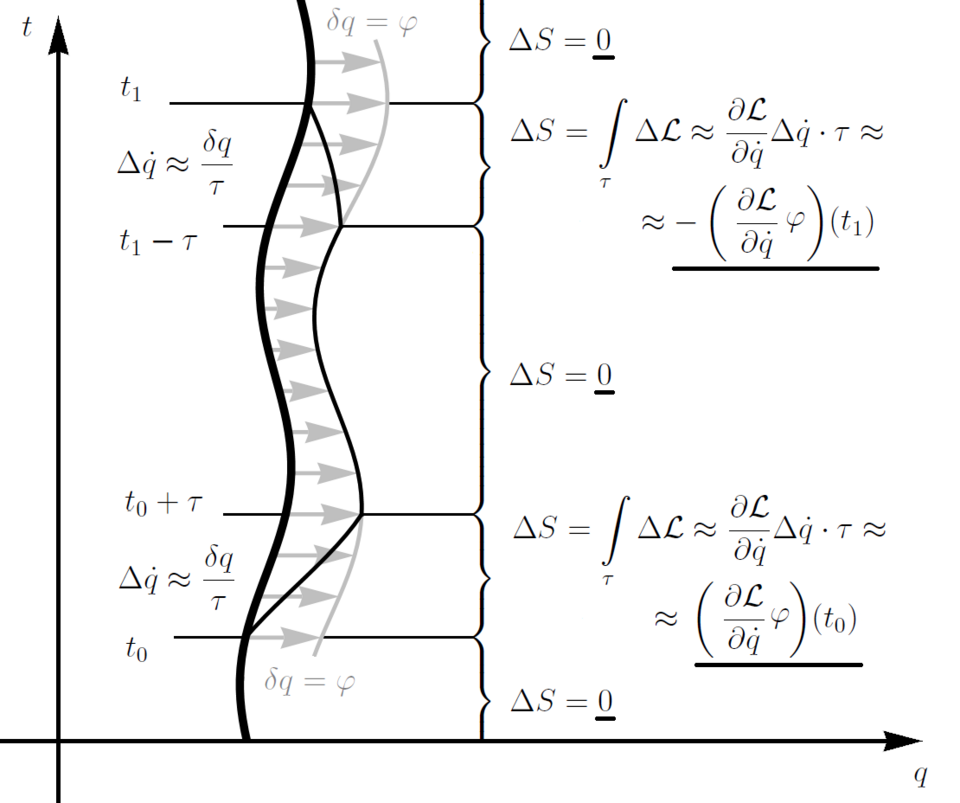
\includegraphics[width=0.75\linewidth]{noether.png}
    \caption{No et ratllis si, de moment, no entens gairebé res d'això. Les matemàtiques del teorema de Noether són difícils fins i tot per a físics i físiques amb molta formació. Foto: L3erdnik, Wikimedia Commons, CC BY 4.0.}
 \end{figure}

Les altres dues simetries també ens porten a lleis de conservació que anirem trobant.

La conservació de la quantitat de moviment ajuda a entendre per què un objecte que viatja per l'espai, si no hi actua cap força externa, no té cap motiu per aturar-se. Si a un astronauta se li escapa una eina, l'eina no pensa ``ja he arribat prou lluny'' i frena educadament.

I la conservació del moment angular és essencial per entendre les rotacions i les òrbites. En un sistema ideal de dos cossos, per exemple, ajuda a mantenir el moviment orbital dins d'un mateix pla.

Per sort, perquè convertir el sistema solar en una coctelera tridimensional complicaria bastant els calendaris.

\subsection{I aquí hi ha la idea important}

Hem començat amb un glaçó, un endoll i una moto fent soroll. Hem acabat parlant de simetries de l'univers.

Pel mig hem trobat una cosa que pot convertir-se en moviment, calor, llum, electricitat o so, però que continua portant els comptes d'una manera sorprenentment estricta.

Aquesta cosa és l'energia.

I potser aquesta és la gràcia de la física: començar preguntant per què s'escalfa una mica d'aigua i acabar descobrint que, darrere de l'experiment, hi havia una propietat de l'espai i del temps esperant tranquil·lament que algú se n'adonés.
